% !TeX root = RJwrapper.tex

\title{TwoSampleTest.HD: An R Ppackage for the Two-Sample Problem with High-Dimensional Data}
\author{by Marta Cousido-Rocha and Jacobo de U\~na-\'Alvarez}

\maketitle

\abstract{
The two-sample problem refers to the comparison of two probability distributions via two independent samples. With high-dimensional data, such comparison is performed along a large number $p$ of possibly correlated variables or outcomes. In genomics, for instance, the variables may represent gene expression levels for $p$ locations, recorded for two (usually small) groups of individuals. In this paper we introduce \CRANpkg{TwoSampleTest.HD}, a new \texttt{R} package to test for the equal distribution of the $p$ outcomes. Specifically, \pkg{TwoSampleTest.HD} implements the tests recently proposed by \cite{Marta2} for the low sample size, large dimensional setting. These tests take the possible dependence among the $p$ variables into account, and work for sample sizes as small as two. The tests are based on the distance between the empirical characteristic functions of the two samples, when averaged along the $p$ locations. Different options to estimate the variance of the test statistic under dependence are allowed. The package \pkg{TwoSampleTest.HD} provides the user with individual permutation $p$-values too, so feature discovery is possible when the null hypothesis of equal distribution is rejected. We illustrate the usage of the package through the analysis of simulated and real data, where results provided by alternative approaches are considered for comparison purposes. In particular, benefits of the implemented tests relative to ordinary multiple comparison procedures are highlighted. Practical recommendations are given.
}

\section{Introduction}\label{se:intro}

%Nowadays a recurring theme is dealing with low sample size and large dimension data  (high-dimensional data). The main property of these high-dimensional data sets is that the data dimension, $p$, i.e., the number of variables or features (e.g. gene expression levels), is large while the sample size is relatively small.

One of the most important questions in modern statistics is how to efficiently deal with the low sample size, high dimensional setting, in which a large number $p$ of variables are measured for a relatively small number of individuals. This type of high-dimensional data arises in many different areas of
science, such as genetics, medicine, pharmacy and social sciences. In microarray data, for example, the variables typically represent the expression levels
of a large set of genes. In such a context, a usual goal is to compare the distributions of the gene expression levels for individuals with two different tumour types. Hence, a formal two-sample test in the 
low sample size and large dimension setting is required. More precisely, the aim is to test for the equality of the
$p$ marginal distributions for the two groups. In other words, one can regard the null hypothesis as the intersection of the $p$ null hypotheses
corresponding to each of the $p$ locations (genes).

In the majority of examples with high-dimensional data the large number of variables or
outcomes are not independent. In genetics, for example, dependency among expression levels of different
genes on the same individual is often observed.
Several two-sample tests have been developed for the high-dimensional setting under dependence; see for instance \cite{BiswasG}, \cite{Mondal}, \cite{Biswaset}, \cite{Liu} and \cite{Wei}. Nevertheless, all of these proposals have at least one of the following disadvantages: (1) the null hypothesis asserts that the $p$-variate distribution is the same
for the two groups being compared instead of testing the equality of
the univariate marginals; (2) the  dependence structure is not considered or is too restrictive; (3) the theoretical results are only suitable for normally distributed data. Besides, to the best of our knowledge none of these methods are available in \texttt{R}. While gaps (2) and (3) are limiting in applications, issue (1) is more fundamental; note that usually the focus is more on the marginal outcome distribution than on the within-group correlation structure. Therefore, new ideas are needed.
%{More precisely, 	\cite{BiswasG},  \cite{Mondal}, and \cite{Biswaset} have the disadvantages (1) and (2) since the dependence structure is modeled  too restrintive.  \cite{Liu} has the disadvantage (2) since the test does not	consider a dependence structure in the high-dimensional data	sets, furthermore they test the equality of the characteristc	functions of the two groups at a given fixed point $t \not =0$,	and the limiting distribution of the test statistic is	derived under the assumption that both the sample size and 	dimension tend to infinity. \cite{Wei} has disadvantage (3) since their theoretical results	are only developed for 	normally distributed data. }






Recently, \cite{Marta2} overcame the aforementioned flaws by introducing a non-parametric omnibus test that, with focus on the marginal distributions, included the dependent case through mixing conditions \citep{Doukhan}. This type of dependence, being fairly general, has been frequently used in
the goodness-of-fit testing literature; see for example \cite{Neu} and
\cite{Deh15}. Mixing conditions imply that the dependence between the variables softens at distant locations. In genetics, for instance, this means that the correlation among expression levels of different genes 
lessens as the distance between the biological function of the genes
increases, which is a flexible, realistic assumption for such applications.

In this paper we introduce the \pkg{TwoSampleTest.HD} \texttt{R} package which implements the tests proposed in \cite{Marta2} for testing the (global, or intersection) null hypothesis of equality of the $p$ univariate marginals
in the two populations. The basic test statistic is the $L_2$-distance between the empirical characteristic functions pertaining to the two groups, when averaged along the $p$ locations. Several approaches to estimate the variance of the test statistic under dependence lead then to slightly different procedures. At the same time, \pkg{TwoSampleTest.HD} provides the user with permutation $p$-values for each location. When the null hypothesis is rejected, these $p$-values can be used to rank the locations according to their contribution to the global significance, or for feature selection by performing multiple testing \citep{Dudoit2007}. Finally, a different test statistic for the global null hypothesis based on the average of the permutation $p$-values is implemented within \pkg{TwoSampleTest.HD}. All of these procedures are fully illustrated in this piece of work.

%Three of the methods are based on a statistic which averages the $p$ individual statistics based on comparing the empirical characteristic functions computed from the two samples, and the difference among the methods is the  approach considered to estimate the variance of such statistic. The last method is an alternative global test whose statistic averages the $p$-values derived from applying permutation tests to the individual statistics mentioned above. When the global null hypothesis is rejected such permutation $p$-values can also be used to identify which variables contribute to this significance.


%\cite{Marta2} methods are the unique test for testing the null hypothesis of the equality of two joint distributions in the high dimensional setting implemented in \texttt{R}. None of the  previous methods mentioned above, as \cite{BiswasG}, \cite{Mondal}, \cite{Biswaset}, \cite{Liu} and \cite{Wei}, have been implemented in an \texttt{R} package.

Alternative nonparametric approaches for the two-sample problem include Kolmogorov-Smirnov and Cramér-von Mises tests. These methods compare the empirical distribution functions, rather than the empirical characteristic functions, of the two groups. Empirical characteristic functions are related to smooth tests, which have been found preferable to distribution-based tests in many settings due to their greater power \citep{MCdUA2009}. More importantly, whenever a test is performed locally and repeatedly, multiple comparison procedures (MCP) are needed in order to keep the type I error under control. Unfortunately, such approach may not be optimal when testing for different distributions in a global way. This relays the fact that feature discovery is more difficult than testing for the intersection null, and explains why the test based on permutation $p$-values implemented in \pkg{TwoSampleTest.HD} can exhibit a power lower than that of the averaged $L_2$-type tests within the package. Efforts to efficiently summarize local $p$-values for testing an intersection null hypothesis include the so-called Higher Criticism (HC) approach, see \cite{Zhangetal2020} and references therein; however, the performance of HC may be dramatically affected by dependence \citep{HallJin2008}. Further discussion of these issues is provided within this paper on the basis of empirical results. 

%the intersection of $p$ null hypotheses corresponding to $p$ different two-sample problems is to test each of the $p$ hypotheses separately via a nonparametric test such as Kolmogorov-Smirnov (KS) or Cramér-von Mises (CvM). Then a multiple comparison procedure (MCP) may be applied to the $p$-values corresponding to the individual tests to check the global null hypothesis. Several R packages implement different MCPs as: the \texttt{stats} package (\texttt{p.adjust} function),  the \texttt{sgof} package \citep{sgof}, the \texttt{multtest} package \citep{multtest} and the \texttt{siggenes} package \citep{siggenes}. Hence, the question here is: Why not follow this approach? The answer is simple, because this approach is less powerfull unless we use an MCP for testing the intersection of the $p$ null hypotheses  and not in determining which of the $p$ null hypotheses should be rejected. The higher-criticism method introduced by \cite{Tukey} is an example of these type of MCPs, unfortunately we are not aware of a similar procedure in the context of dependent data.






The rest of the paper is organized as follows. In Section \ref{se:metho} the methodological background is
introduced, and the tests proposed by \cite{Marta2}
are presented in detail. In Section \ref{se:pra} the \pkg{TwoSampleTest.HD} package is described, and its usage is illustrated
through the analysis of simulated data and microarray data  derived from a hereditary breast cancer study. Finally, Section \ref{se:con} reports the main conclusions of this work.


\section{Methodology}\label{se:metho}

In this section we describe the four two-sample tests proposed by \cite{Marta2}, which are implemented in the \pkg{TwoSampleTest.HD} package. Three of the methods are based on the
average of $p$ individual $L_2$-distances between the empirical characteristic functions
computed from the two samples. The three versions of this test differ in the way in which the variance is estimated; in all the cases, the variance estimate takes the possible dependence among the $p$ outcomes into account. The fourth method is based on the average of the permutation $p$-values derived for the individual $L_2$-distances.


We consider two random matrices  $X=\left[X_1, \dots, 
X_p\right]^T$ and $Y=\left[Y_1, \dots, Y_p\right]^T$ of respective 
dimensions $p \times n$ and $p \times m$, where
$X_k=(X_{k1}, \dots,$ $X_{kn})$ and $Y_k=\left(Y_{k1}, \dots,
Y_{km}\right)$, $k=1, \dots,p$, are the sample values for the $p$ target variables; the sample sizes are $n$ and $m$. The variables $X_k$ and $Y_k$ may be discrete or continuous; normality is not assumed in the continuous case. Given sequences of characteristic functions $\{C_{X_1}, C_{X_2},\ldots, C_{X_p}\}$ and
$\{C_{Y_1}, C_{Y_2},\ldots, C_{Y_p}\}$, it is assumed that $X_{k1}, \dots, 
X_{kn}$ and $Y_{k1},\ldots,Y_{km}$ are independent random samples from
$C_{X_k}$ and $C_{Y_k}$, respectively. Observations 
$X_{ij}$ and $X_{sl}$ for $s\not =i$  can be dependent in our
framework, and similar comments apply to the components of
$Y$. 

The focus is in testing for the intersection null hypothesis  
$$ H_0= \bigcap_{k=1}^{p}  H_{0k},$$
where, for $1 \leq k \leq p$, $H_{0k}$ states that $C_{X_k}$ and $C_{Y_k}$ coincide. As indicated by \cite{Marta2}, the $L_2$-distance between the empirical characteristic functions of $X_k$ and $Y_k$ is given by

\begin{eqnarray}\label{ec:jk}
	\nonumber	J_k&=& \dfrac{1}{n(n-1)} \sum_{j=1}^{n} \sum_{l=1, l \not =
		j}^{n} \exp\left(-\dfrac{1}{2}\left(\dfrac{X_{kj}-X_{kl}}{\sqrt{2}b}\right)^2\right)\\&+& \nonumber\dfrac{1}{m(m-1)} \sum_{j=1}^{m} \sum_{l=1, l \not =
		j}^{m} \exp\left(-\dfrac{1}{2}\left(\dfrac{Y_{kj}-Y_{kl}}{\sqrt{2}b}\right)^2\right)\\&-&
	\dfrac{2}{nm}\sum_{j=1}^{n} \sum_{l=1}^{m} \exp\left(-\dfrac{1}{2}\left(\dfrac{X_{kj}-Y_{kl}}{\sqrt{2}b}\right)^2\right),
\end{eqnarray}
where $b \in \mathbb{R}^{+}$. The first term in $J_k$ is an intra-sample parameter
estimate for the sample $X_k$ and the second term is an intra-sample
parameter estimate for the sample $Y_k$,  whereas the third term is an
{\it inter}-samples parameter estimate, since $X_{kj}$  and $Y_{k\ell}$ come
from different samples, $X_k$ and $Y_k$, respectively. 

%{\color{blue} Each of the two-sample tests based on the statistics in (\ref{ec:jk}) is introduced below, it is important to note that all of them are generally applicable to continuous or discrete populations, both Gaussian and non-Gaussian.}

We consider the test statistic $T_p=\sum_{k=1}^{p} J_k/\sqrt{p}$ in order to test for $H_0$. \cite{Marta2} introduced two variance estimators for $T_p$
when $(X_k,Y_k)_{k \in \{1, \dots, p\}}$ comes from a strictly stationary 
sequence  $(X_k,Y_k)_{k\in\mathbb{N}}$. The first variance estimator $\widehat \sigma_S$ is based on the spectral density estimate. Indeed, the problem of estimating the
variance of a sample mean based on dependent data is the same as that of estimating the
spectrum of the process at frequency zero. Hence, Var($T_p$) can be approximated through the
classical estimator of the spectrum of the process at frequency zero. It holds that $T_p/\widehat{\sigma}_S \overset{D}{\longrightarrow} \mathcal{N}(0,1)\;\; \text{as} \; p \; \text{tends to} \; \infty.$ 
Since the expectation of $T_p$ is strictly positive under the alternative hypothesis, the test is one-sided, and rejects $H_0$ at nominal level $\alpha$ when $T_p/\widehat{\sigma}_S$ is larger than
the $1-\alpha$ quantile of the standard normal distribution. We refer to this test as spectral test.

The second variance estimator is derived from the block bootstrap procedure proposed by \cite{Carls} to estimate the variance
of a general statistic computed from a strictly stationary $\alpha$-mixing
sequence \citep[see][]{Bosq}. More precisely, this resampling method defines no overlapping blocks of length $l$ on the sequence 
$(J_k)_{k \in \{1, \dots, p\}}$ and computes the statistic $T_p$ in each of the blocks, with $l$ being the maximum lag of significant autocorrelation on the $(J_k)_{k \in \{1, \dots, p\}}$ sequence according to the procedure in \cite{PoW}. Finally the  block bootstrap variance estimator $\widehat \sigma_B$ is simply defined as the sample variance of the values of $T_p$ in each of the block. As before, the standardized version of $T_p$ based on  $\widehat{\sigma}_B$, is asymptotically distributed as a $\mathcal{N}(0,1)$ random variate. Hence, 
the block bootstrap test rejects the null hypothesis when $T_p/\widehat{\sigma}_B$ is larger than the $1-\alpha$
quantile of the standard normal distribution.


\cite{Marta2} also introduced
an alternative variance estimator suitable for
possibly non-stationary sequences based on $U$-statistics theory. More precisely, the variance of $T_p$ can be written as the sum of two terms; the first one is the average of the variance of the statistics $(J_k)_{k \in \{1, \dots, p\}}$, whereas the second one comprises the covariance terms arising from such sequence. The first term can be estimated by replacing the unknown theoretical expectations by their corresponding sample means; on the other hand, an unbiased estimator for the covariance term ${Cov}(J_j,J_{j+k})$ is given by $J_jJ_{j+k}$, $j=1, \dots, p-l$, $k=1, \dots, l$.  The standardized version of $T_p$ based on such variance estimator, $T_p/\widehat{\sigma}_U$, is asymptotically distributed as a $\mathcal{N}(0,1)$ as $p \rightarrow \infty$. Hence, 
the $U$-statistic test rejects the null hypothesis when $T_p/\widehat{\sigma}_U$ is larger than the $1-\alpha$
quantile of the standard normal distribution.


Interestingly, the test statistics $J_k$ can be used locally to test for the null
hypotheses $H_{0k}$ that $X_{k1}$ and $Y_{k1}$ have the same
distribution, $1\leq k\leq p$. Since the  common density under $H_{0k}$ is unknown, a permutation test can be used to calibrate the null distribution of $J_k$. The application of the permutation test to each of the $H_{0k}$, $k\in\{1,\ldots, p\}$ yields a set of $p$-values $\{P_1,
\ldots, P_p\}$. \cite{Marta2} proposed a test statistic based on the average of the permutation $p$-values, $\bar P=\sum_{k=1}^{p}
P_k/p$.  The idea of combining  the individual
$p$-values to obtain a global test statistic is old, dating
to \cite{Fisher,stou} and others. The statistic $P$ is standardized taking into account that its expectation is ${(N+1)}/{2N}$, with $N$ being the number of permutations that lead to a different value of the statistic $J_k$, and using a variance estimator based on the spectral analysis. 
The standardized version of $\bar P$, say $T_p^{pv}={\sqrt{p}\left(\bar 
	P-(N+1)/(2N)\right)}/{\widehat{\sigma}_{P}}$, is asymptotically distributed as a standard normal as $p \rightarrow \infty$. It is assumed that, under $H_0$,  $(X_k,Y_k)_{k \in \{1, \dots, p\}}$ comes from a strictly stationary and  strongly mixing 
process  $(X_k,Y_k)_{k\in\mathbb{N}}$. The null hypothesis is rejected when $T_p^{pv}$ is smaller than the $\alpha$
quantile of the standard normal distribution. One advantage of the permutation $p$-values is that, when the intersection null is rejected, they can be used to rank
the null hypotheses $H_{0k}$ according to their contribution to the
significance. In genomics, for instance, this ranking may reveal the genes which express differently 
between two tumors. 
Finally, a formal MCP can be applied to the set of permutation $p$-values to get rigorous conclusions
on the individual nulls $H_{0k}$, $k\in\{1,\ldots, p\}$. {Note that the ranking provided by the $p$-values is related, but not equal, to the ranking based on the $J_k$'s; this is because the target outcome may be differently distributed along the $p$ locations, and $J_k$ is not distribution free. The situation for the Hedenfalk data example in Section \ref{se:he} is depicted in Figure \ref{figanti}; the shift of the $p$-values distribution compared to uniform suggests that some genes are differently expressed in the two groups considered.}

\begin{figure}[htb]
	\centering
	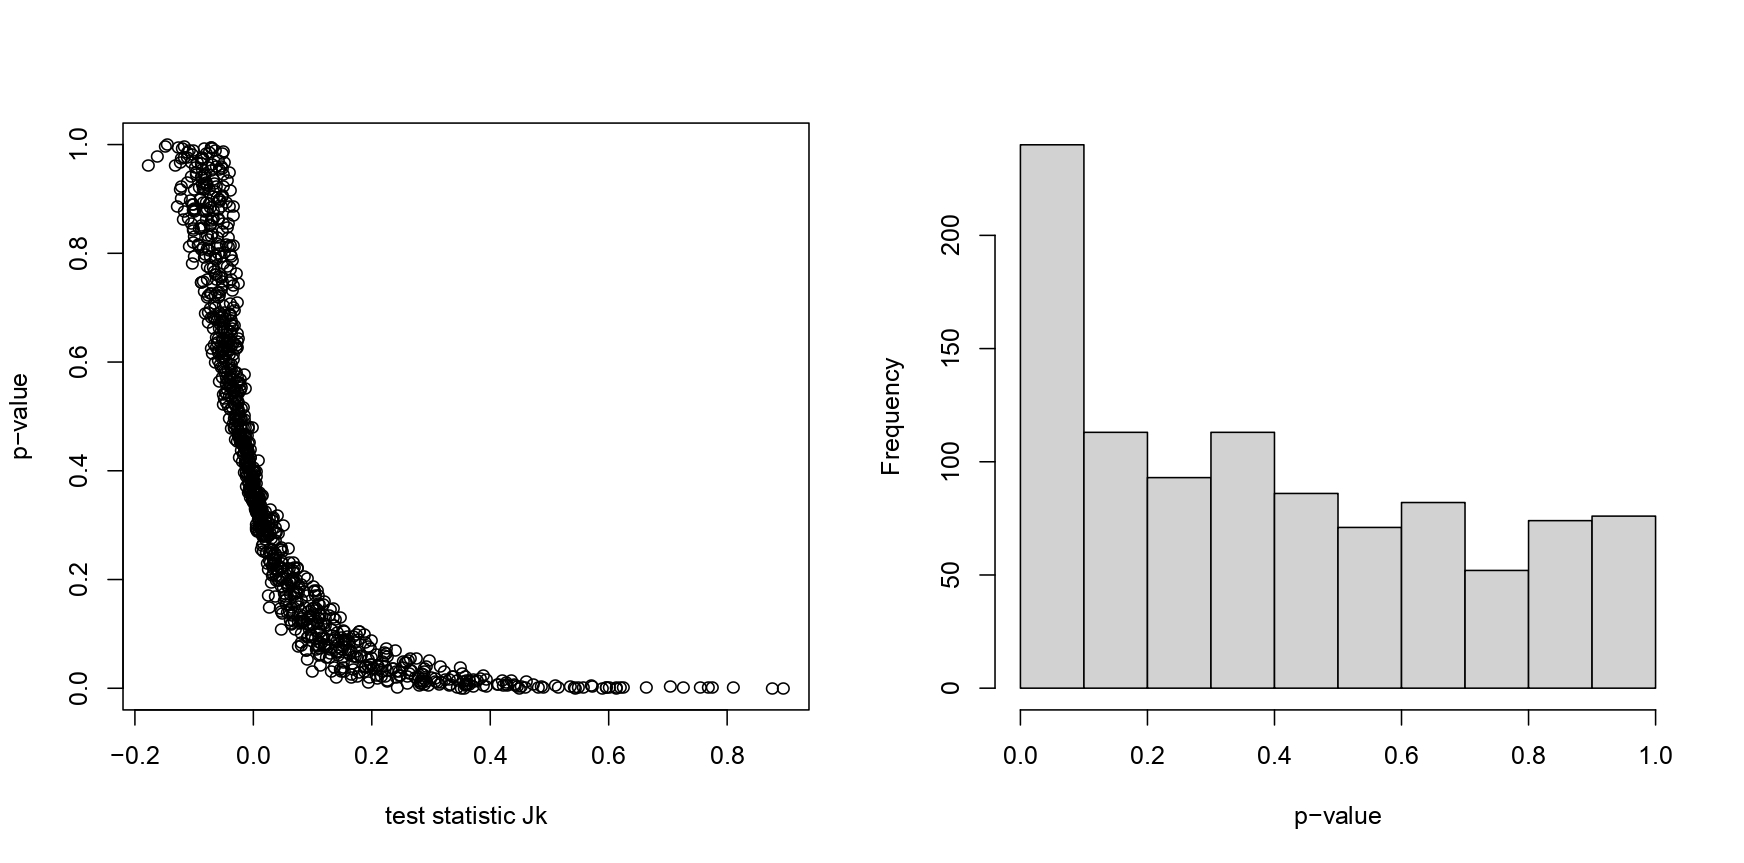
\includegraphics[width=1\textwidth]{figanti.jpg}
	\caption{Left: $p$-values vs test statistics $J_k$. Right: histogram of the $p$-values. Hedenfalk data.}
	\label{figanti}
\end{figure}

For the implementation of the aforementioned test statistics the parameter $b$ in (\ref{ec:jk}), which plays the role of a smoothing parameter or bandwidth, is set to  $\widehat{b}=1.144 s_{pool} \left(({n+m})/{2}\right)^{-1/5},$
where $s_{pool}^2$ is the average of
$\left((n-1)s_{X_k}^2+(m-1)s_{Y_k}^2)\right)/(n+m-2)$, $k=1, \dots,p$, and
$s_{X_k}^2$ and $s_{Y_k}^2$ are the sample variances of $X_k$ and
$Y_k$, respectively, $k=1, \dots, p$. When the permutation $p$-values of the statistics $J_k$ are to be computed, a local bandwidth can be used instead; specifically, the local bandwidth for $J_k$ is given by $\widehat{b}_k=1.144 s_{pool} \left(({n+m})/{2}\right)^{-1/5},$ with $s_{pool}^2=\left((n-1)s_{X_k}^2+(m-1)s_{Y_k}^2)\right)/(n+m-2)$, and $s_{X_k}^2$ and $s_{Y_k}^2$ are the sample variances of $X_k$ and
$Y_k$.

\section{Package \pkg{TwoSampleTest.HD} in practice}\label{se:pra}

In this section the main features of \pkg{TwoSampleTest.HD} package are described.  We also consider two examples with high-dimensional data in order to explain how to use \pkg{TwoSampleTest.HD} in practice. The first example refers a large number of gene expression levels measured on two groups of patients
with breast cancer, classified according to BRCA mutation type.  The
second example is a simulation scenario in which the target outcome is differently distributed in the two groups for 10\% of the $p$ locations. This second example serves in particular to illustrate the smaller power of ordinary MCP when compared to the tests based on the averaged $L_2$-distances between the empirical characteristic functions of the two groups.


\subsection{Hedenfalk data}\label{se:he}

In this subsection we consider the microarray data set of
hereditary breast cancer in \cite{He}. The data set
consists of $p=3226$ logged gene 
expression levels measured on
$n=7$ patients with breast tumors
having BRCA1 mutations and on $m=8$
patients with breast tumors
having BRCA2 mutations. The goal is to test the null
hypothesis that the distribution of the $p$ genes is the same
for the two types of tumor, BRCA1 tumor 
and BRCA2 tumor. Since the example is merely illustrative, we only consider the first 1000 genes in order to save computational time. With 1000 locations, the execution time is reduced to $<$ 1 second for the block bootstrap and spectral tests, to $<$ 5 seconds for the $U$-statistic test and to 9 minutes for the permutation $p$-values test,  in a laptop provided
	with a i5-1135G7 CPU. The waiting time of the  permutation test is relatively long since  $n=7$ and $m=8$ lead to $6435$ permutations which must be carried out for each of the $p=1000$ genes. For additional inspection, in Table \ref{ca:time} execution times for simulated data with several dimensions $p$ and sample sizes $n$ and $m$ are reported.

\begin{table}[]
		\begin{center}
	\begin{tabular}{lllllll}
	\hline	& \multicolumn{3}{l}{Spectral}      & \multicolumn{3}{l}{Block bootstrap} \\
		$p/n, m$ & $2,2$     & $5,5$     & $10,10$   & $2,2$     & $5,5$     & $10,10$     \\
		100      & 0.01      & 0.02      & 0.01      & 0.01      & 0.02      & 0.03        \\
		500      & 0.03      & 0.03      & 0.06      & 0.03      & 0.05      & 0.10        \\
		1000     & 0.07      & 0.08      & 0.11      & 0.07      & 0.07      & 0.12        \\
	\hline	& \multicolumn{3}{l}{$U$-statistic} & \multicolumn{3}{l}{Permutation}     \\
		$p/n, m$ & $2,2$     & $5,5$     & $10,10$   & $2,2$     & $5,5$     & $10,10$     \\
		100      & 0.01      & 0.11      & 0.58      & 0.03      & 0.89      & 1182.40     \\
		500      & 0.11      & 0.57      & 2.51      & 0.015     & 3.55      & 5122.53     \\
		1000     & 0.24      & 1.04      & 4.87      & 0.27      & 8.13      & 8006.70  \\
		\hline  
	\end{tabular}
\end{center}
\caption{Execution time (in seconds) for the several versions of the proposed two-sample test. Simulated data with dimension $p$ and sample sizes $n$ and $m$.}	
\label{ca:time}
\end{table}


The main function of the package is \pkg{TwoSampleTest.HD}.
This function computes, among other things, the value of the selected test statistic and the corresponding $p$-value. The list of arguments of \pkg{TwoSampleTest.HD} is given in Table \ref{ca:argu}. The required arguments are 
\texttt{X} and \texttt{Y}, matrices where each row is one of the $p$-samples in the first group and second group, respectively; the other arguments have a default value. When the user forgets to include the
argument \texttt{X} or \texttt{Y} in the function, the following message is returned:

\begin{example}
	Call: 
	TwoSampleTest.HD(X = X)
	'us' method used by default
	'global' bandwidth used by default
	Error in ncol(Y) : argument "Y" is missing, with no default
\end{example}

\begin{example}
	Call: 
	TwoSampleTest.HD(Y= Y)
	'us' method used by default
	'global' bandwidth used by default
	Error in ncol(X) : argument "X" is missing, with no default
\end{example}


With \texttt{method="spect"} the two-sample spectral test described in Section \ref{se:metho} is applied; the option  \texttt{"method=spect$\_$ind"} corresponds to a simplified version that pre-assumes the independence among the outcomes. On the other hand, the options \texttt{method="us"} and \texttt{method="us$\_$ind"} apply the two-sample $U$-statistic test explained in Section \ref{se:metho} for dependent data  and its simplification for independent variables, respectively. The last option based on the average of the $p$ individual
statistics, $J_k$, corresponding to each of the $p$ variables is \texttt{method="boot"} which implements the two-sample block bootstrap test (Section \ref{se:metho}). Finally, the function also performs the alternative test based on the average of the
permutation $p$-values corresponding to the individual statistics $J_k$ through the argument \texttt{method="perm"}.
In our experience, the most powerful test for independent outcomes is the $U$-statistic test,
whereas under dependence the more powerful tests are the spectral and
block bootstrap tests. We also observed that the block
bootstrap and spectral tests, which were developed
assuming that $(X_k,Y_k)_{k\in\mathbb{N}}$ is a strictly stationary
process, performed well when stationarity is violated. The \texttt{"us"} method  has been defined as the default one.

When choosing \texttt{method="perm"}, the sequence of permutation $p$-values is computed and reported. On the other hand, the computation of the permutation $p$-values must be explicitly requested using \texttt{I.permutation.p.values=TRUE} argument for the $U$-statistic, spectral or block bootstrap tests.  As mentioned, these individual $p$-values may be used to rank the outcomes according to their significance. Argument \texttt{b$\_$I.permutation.p.values} allows the user to select the bandwidth $b$. The option \texttt{b$\_$I.permutation.} \texttt{p.values="global"} computes a global bandwidth $\widehat{b}$ and uses it to evaluate the $J_k$'s, whereas option \texttt{b$\_$I.permutation.p.values="individual"} 
estimates the bandwidth  for each variable separately; see details in Section \ref{se:metho}. The default option is \texttt{b$\_$I.permutation.p.values="global"}. In Table \ref{ca:re} a summary of the results provided by the function \pkg{TwoSampleTest.HD} is given. The \texttt{I.statistics}
object contains the individual statistics $J_k$ , $k = 1, \dots, p$ described in the previous section, while the \texttt{I.permutation.p.values} object reports the 
permutation $p$-values $\{P_1,
\ldots, P_p\}$.
%\addtolength{\tabcolsep}{-5pt}

%In this way if the global null hypothesis is rejected the user has a sequence of $p$-values which can be employed  to rank the null hypotheses $H_{0k}$ according to their contribution to the significance. For example, in genomics we can rank the genes using the $p$-values to infer which genes express differently  between two tumors.  This ranking is an exploratory device. On the other hand the application of a multiple comparison procedure (MCP) to the set of $p$-values is a rigorous procedure to test each $H_{0k}$, $k=1, \dots, p$.


	\begin{table}
	\begin{center}
		\begin{tabular}{ll}
			\hline
			{Usage of the function}:  &   \\
			& \hspace{-10cm}\begin{lstlisting}
				TwoSampleTest.HD(X, Y, method = c("spect",
				"spect_ind", "boot", "us","us_ind", "perm"), 
				I.permutation.p.values = FALSE,
				b_I.permutation.p.values = c("global", "individual"))
		\end{lstlisting}\\
			& \\
			\hline
			& \\
		\hspace{-8cm}
				\begin{lstlisting}
					X  
				\end{lstlisting}
				 & \hspace{-0.25cm}\begin{tabular}{l}A matrix where each row is one of the $p$-samples\\
				in the first group.\end{tabular}\\
			\hspace{-8cm}
				\begin{lstlisting}
					Y
				\end{lstlisting} 
			 & \hspace{-0.25cm}\begin{tabular}{l}A matrix where each row is one of the $p$-samples\\
				in the second group.\end{tabular} \\
		\hspace{-8cm}
				\begin{lstlisting}
					method
				\end{lstlisting}
				 & \hspace{-0.25cm}\begin{tabular}{l}
				The two-sample test. By default the ``us'' method \\
				is computed.
				%Note that ``us'' refers to the U-statistic test introduced in Section \ref{se:metho}.
			\end{tabular}\\
			\hspace{-8cm}
				\begin{lstlisting}
					I.permutation.p.values
				\end{lstlisting}
			 & \hspace{-0.25cm}\begin{tabular}{l}Logical. Default is FALSE. A variable indicating\\
				whether to compute the permutation $p$-values or \\
				not when the selected method is not ``perm''. \\
				%Note that ``perm'' refers to the global test based on permutation\\
				%$p$-values introduced in Section \ref{se:metho}.
			\end{tabular}\\
		\hspace{-8cm}
				\begin{lstlisting}
					b_I.permutation.p.values
				\end{lstlisting}  & \hspace{-0.25cm}\begin{tabular}{l} The bandwidth method used to compute the\\ individual
				statistics on which are based the\\ permutation
				$p$-values.\end{tabular}\\
			\hline
		\end{tabular}   
		\caption{Usage and list of the arguments of the  \pkg{TwoSampleTest.HD} function.}
		\label{ca:argu}
	\end{center}
\end{table}





\begin{table}[htb]
	\begin{center}
		\begin{tabular}{ll}
			\hline
			\hspace{-6cm}	\begin{lstlisting}	
				standardized statistic
			\end{lstlisting} &
			the value of the standardized statistic.\\
			\hspace{-6cm}	\begin{lstlisting}
				p.value
			\end{lstlisting} & the $p$-value for the test.\\
			\hspace{-6cm}	\begin{lstlisting}
				statistic
			\end{lstlisting} & the value of the statistic.\\
			\hspace{-6cm}	\begin{lstlisting}
				variance
			\end{lstlisting}& the value of the variance estimator.\\
			\hspace{-6cm}	\begin{lstlisting}
				p
			\end{lstlisting}& number of samples or populations.\\
			\hspace{-6cm}	\begin{lstlisting}
				n
			\end{lstlisting}& sample size in the first group.\\
			\hspace{-6cm}	\begin{lstlisting}
				m
			\end{lstlisting}& sample size in the second group.\\
			\hspace{-6cm}	\begin{lstlisting}
				method
			\end{lstlisting}& a character string indicating which two sample test is performed.\\
			\hspace{-6cm}	\begin{lstlisting}	
				I.statistics
			\end{lstlisting}& the $p$ individual statistics.\\
			\hspace{-6cm}	\begin{lstlisting}	
				I.permutation.p.values
			\end{lstlisting}& the $p$ individual permutation $p$-values.\\
			\hspace{-6cm}	\begin{lstlisting}	
				data.name
			\end{lstlisting}& a character string giving the name of the data.\\
			\hline
		\end{tabular}
	\end{center}
	\caption{Summary of the results reported by \pkg{TwoSampleTest.HD} function.}
	\label{ca:re}
\end{table}

Hedenfalk data are available within \CRANpkg{Equalden.HD} package \citep{CRdUA_CMPB}. In order to analyze this dataset,
we load this package together with \pkg{TwoSampleTest.HD} package. For the investigation of the possible dependence among the gene expression levels, we treat the data of each patient as a time series, and we compute the
sample autocorrelation function. For the first lags the autocorrelation
between genes was significantly different from zero, whereas it lessened
as the number of lags increased. The estimates of the autocorrelation were computed using the \texttt{acf} function of the R package \CRANpkg{stats}. On the basis of these results, the weak dependence assumption behind the  tests implemented in  the \pkg{TwoSampleTest.HD} seems realistic. The four tests designed for weak dependence (spectral test, $U$-statistic test, block bootstrap test and permutation test) can be performed by using the following code lines:

\begin{example}
	> library(Equalden.HD)
	> data("Hedenfalk")
	> X=log(Hedenfalk[,1:7])
	> Y=log(Hedenfalk[,8:15])
	> 
	> X=X[1:1000,]
	> Y=Y[1:1000,]
	> library(TwoSampleTest.HD)
	> res1 <- TwoSampleTest.HD(X, Y, method = "spect")
	Call: 
	TwoSampleTest.HD(X = X, Y = Y, method = "spect")
	'global' bandwidth used by default
	
	A two-sample test for the equality of distributions for high-dimensional data
	
	data:  c(X, Y)
	standardized statistic = 11.536, p-value < 2.2e-16
	
	> res2 <- TwoSampleTest.HD(X, Y, method = "boot")
	Call: 
	TwoSampleTest.HD(X = X, Y = Y, method = "boot")
	'global' bandwidth used by default
	
	A two-sample test for the equality of distributions for high-dimensional data
	
	data:  c(X, Y)
	standardized statistic = 11.515, p-value < 2.2e-16
	
	> res3 <- TwoSampleTest.HD(X, Y, method = "us")
	Call: 
	TwoSampleTest.HD(X = X, Y = Y, method = "us")
	'global' bandwidth used by default
	
	A two-sample test for the equality of distributions for high-dimensional data
	
	data:  c(X, Y)
	standardized statistic = 12.104, p-value < 2.2e-16
	
	> res4 <- TwoSampleTest.HD(X, Y, method = "perm")
	Call: 
	TwoSampleTest.HD(X = X, Y = Y, method = "perm")
	'global'bandwidth used by default
	
	A two-sample test for the equality of distributions for high-dimensional data
	
	data:  c(X, Y)
	standardized statistic = -10.955, p-value < 2.2e-16
	
\end{example}


The output of the function \pkg{TwoSampleTest.HD} shows that $T_p/\widehat{\sigma}_S=11.536$, $T_p/\widehat{\sigma}_B=11.515$, $T_p/\widehat{\sigma}_U=12.104$ and
$T_p^{pv}=-10.955$, whereas the
corresponding $p$-values are almost zero. The negative value of the $T_p^{pv}$ statistic means that the average of the permutation $p$-values is lower than the expected mean of their (uniform) null distribution. Hence, the null hypothesis is rejected; the conclusion is that one or
more genes are differently expressed depending on the tumor type. The object derived from \pkg{TwoSampleTest.HD} function is a list which saves, as usual with \texttt{R} functions, relevant information. Besides the standardized statistic and the $p$-value printed in the console when running the function (as shown above), the list of saved objects comprises
the value of the statistic $T_p$ (or $\sqrt{p}\bar 
P$ if one runs the permutation test), the variance ($\widehat{\sigma}_S$, $\widehat{\sigma}_B$, $\widehat{\sigma}_U$ or $\widehat{\sigma}_{P}$), the number of variables ($p$), the sample sizes ($n$ and $m$), the method used
for the data analysis, and the values of the statistics $J_1, \dots, J_p$. 
Below, we display such information for the spectral test as an illustrative example. The values of the statistics  $J_1, \dots, J_p$ are plotted in Figure \ref{fig:1} instead  of reporting them through the console. 

\begin{example}
	> res1\$statistic
	[1] 1.827471
	> res1\$variance
	[1] 0.02509699
	> res1\$p
	[1] 1000
	> res1\$n
	[1] 7
	> res1\$m
	[1] 8
	> res1\$method
	[1] "spect"
	> library(ggplot2)
	> 
	> data=data.frame(Jk=res1\$I.statistics,Genes=1:res1\$p)
	> ggplot(data, aes(x=Genes, y=Jk)) +
	+   geom_point(shape=21, col=8) + geom_rug()+ggtitle("Individual test statistics")
\end{example}




\begin{figure}[htb]
	\centering
	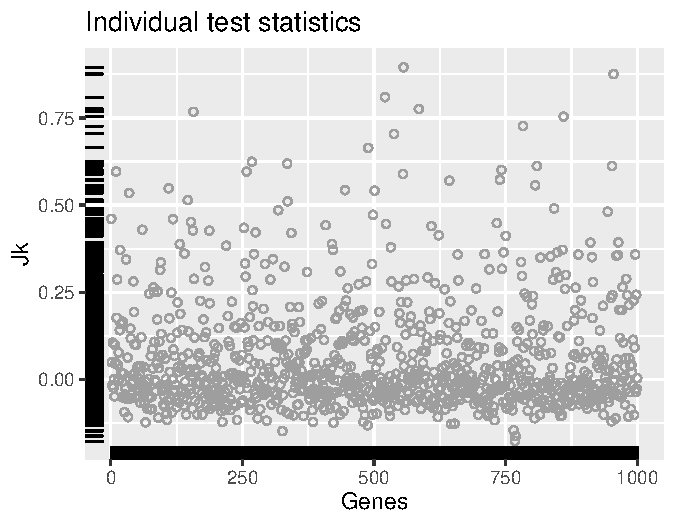
\includegraphics[width=1\textwidth]{ima1.pdf}
	\caption{The values of the statistics $J_1, \dots, J_p$ for the two-sample spectral test. Hedenfalk data.}
	\label{fig:1}
\end{figure}


Since the null hypothesis is rejected for Hedenfalk data, the next natural aim is to identify which genes are not equally distributed in both types of tumors. For this, we first rank
the null hypotheses $H_{0i}$ according to their contribution to the
significance by using the sequence of permutation $p$-values. This sequence has only been computed for the permutation test, since for the remaining tests it is only computed when the argument \texttt{I.permutation.p.values} is equal to \texttt{TRUE} and, in our previous applications of the tests such argument has not been specified hence the default option \texttt{I.permutation.p.values=FALSE} has been used. Therefore, \texttt{res4} is the unique object which has the sequence of permutation $p$-values. Note that, since the argument \texttt{b$\_$I.permutation.p.values} has not been used, the default option \texttt{b$\_$I.permutation.p.values="global"} has been considered, and then the global $\widehat{b}$ has been employed to compute each one of the $J_k$, $k=1, \dots, p$, for which the permutation $p$-values are calculated. Below, the code used to determine which are the 10 genes of lowest $p$-values is reported.

\begin{example}
	> pv=res4\$I.permutation.p.values
	> order(pv)[1:10]
	[1] 556 733 952 955 445 555 914 963 118 157
\end{example}


Although the above list can be informative, any rigorous procedure should keep the type I error under control. The \texttt{p.adjust} function, available within \pkg{stats} package, implements the well-known \cite{BH} false discovery rate (FDR) controlling procedure. The application of this method to the sequence of 1000 permutation $p$-values at 5\% FDR level reports 13 discoveries (see code lines below). Note that, although \cite{BH} has been initially studied for independent $p$-values, subsequent research has shown that it remains valid under weaker assumptions.

\begin{example}
	> alpha=0.05
	> sum(p.adjust(pv,method = "BH")<=alpha)
	[1] 13
	
\end{example}



One interesting question is whether nonparametric two-sample test statistics alternative to $J_k$ could perform better in the multiple testing setting. As a by-product of their research, \cite{Marta3} proved through simulations  that the $J_k$ test statistic performs similarly or even better than other well-known two-sample tests. For example, simulation results in the referred paper suggest that the Kolmogorov–Smirnov test should not be used when the sample sizes are small and the
differences are other than location. For illustrative purposes, we have tested each one of the null hypothesis  $H_{0k}$, $k\in\{1,\ldots, p\}$, through 
Student's t test, Wilcoxon test, Levene test and Kolmogorov-
Smirnov test (see \citealp{Gi} and \citealp{le}). Then,
\cite{BH} has been applied to the corresponding $p$-values sequence (code below).


\begin{example}
	> p=res1\$p;n=res1\$n; m=res1\$m
	> pv_t.test=1:p
	> pv_KS=1:p
	> pv_Wilcoxon=1:p
	> pv_Levene=1:p
	> 
	> library(car)
	> library(exactRankTests)
	> library(coin)
	> 
	> for (i in 1:p){
		+   pv_Wilcoxon[i]=wilcox.exact(X[i,],Y[i,])\$p.value
		+   pv_t.test[i]=t.test(X[i,],Y[i,],var.equal = F)\$p.value
		+   pv_KS[i]=ks.test(X[i,],Y[i,])\$p.value
		+   pv_Levene[i]=leveneTest(c(X[i,],Y[i,]),
		+   as.factor(c(rep(1,n),rep(2,m))))\$`Pr(>F)`[1]
		+ }	
	> sum(p.adjust(pv_Wilcoxon,method = "BH")<=alpha)
	[1] 13
	> sum(p.adjust(pv_t.test,method = "BH")<=alpha)
	[1] 1
	> sum(p.adjust(pv_KS,method = "BH")<=alpha)
	[1] 0
	> sum(p.adjust(pv_Levene,method = "BH")<=alpha)
	[1] 0
\end{example}

From results above it is seen that the Kolmogorov–Smirnov (KS) test is unable to provide any discovery at 5\% of FDR. However, these results should be taken with some caution since exact KS $p$-values could not be computed by \texttt{ks.test} function due to the presence of ties in Hedenfalk data; note that the asymptotic distribution of the KS test may be inaccurate for small sample sizes. The lack of power of  KS in the multiple testing setting has been pointed out in \cite{Marta3} too. Similarly as for KS, Levene test does not declare any gene as differently expressed in the two tumor groups; this is not surprising, since differences between the two groups are mainly due to a location shift \citep{He}. The number of discoveries of the $t$-test is very low (only one rejection); on the contrary, Wilcoxon test provides as many discoveries as the $J_k$ test statistic. In order to better summarize the relative power of the several testing procedures, Figure \ref{fig:2} depicts the number of rejections along a sequence of nominal levels for the FDR ($\alpha = 0.001, 0.002, \dots, 0.10$). Interestingly, Figure \ref{fig:2} supports previous comments on the poor performance of KS test.



\begin{figure}[htb]
	\centering
	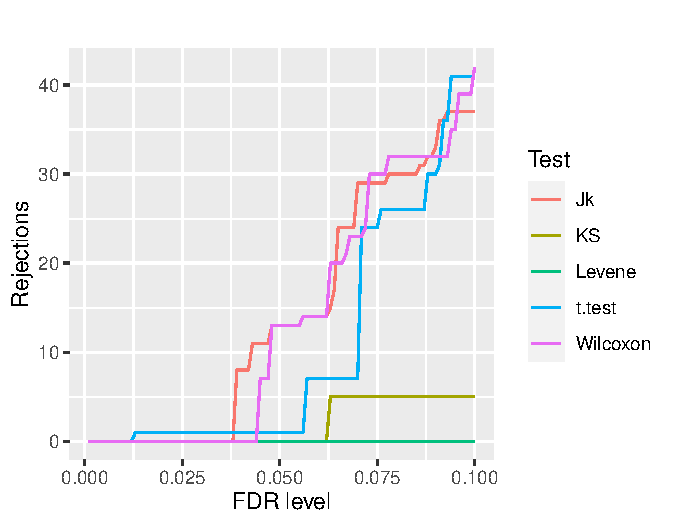
\includegraphics[width=1\textwidth]{ima2.pdf}
	\caption{Number of rejections of Wilcoxon test, Kolmogorov-Smirnov test, $t$-test, Levene test and $J_k$ permutation test depending on the nominal FDR level. Hedenfalk data.}
	\label{fig:2}
\end{figure}

\subsection{Simulated data}\label{se:simul}

%In this section simulated data is  analyzed using the \pkg{TwoSampleTest.HD} package. The main aim is to illustrate in a simulating scenario  the power limitations of testing the intersection of the $p$ null hypotheses (global null) testing each of the $p$ hypotheses separately (applying a MCP over the sequence of $p$-values).


We simulated $p=1000$ independent variables with sample sizes $n=m=4$ under the alternative hypothesis. More precisely, the $p$ samples in the first group ($X$) were generated in 4 blocks from  the following distributions, respectively:
$N(0,1)$, $N(0,2)$, $N(1,1)$ and $N(1,2)$. In the second group ($Y$), $90\%$ of the $p$ samples were generated exactly as for $X$ (true individual nulls), whereas for simulating the remaining $10\%$ of the samples the distributions were interchanged, with a location shift as result (non-true individual nulls). To be specific, in the case $X \sim N(0,1)$, the $Y$ was generated from a $N(1,1)$, and vice versa; when $X \sim N(0,2)$, the $Y$ was generated from a $N(1,2)$, and vice versa. The code for the simulation is provided in Appendix \ref{appendix}.

Below, the two-sample tests implemented in \pkg{TwoSampleTest.HD} are applied to test the null
hypothesis that the distribution of each of the samples is the same in the groups. All of the tests reject the null hypothesis. The results suggest that the simpler versions which make use of the independence assumption, \texttt{"spect\_ind"} and \texttt{"us\_ind"}, are slightly more powerful than their counterparts for dependent data.

\begin{example}
	> TwoSampleTest.HD(X, Y, method = "spect")\$p.value
	Call: 
	TwoSampleTest.HD(X = X, Y = Y, method = "spect")
	'global' bandwidth used by default
	
	A two-sample test for the equality of distributions for high-dimensional data
	
	data:  c(X, Y)
	standardized statistic = 2.2275, p-value = 0.01296
	
	[1] 0.01295652
	> TwoSampleTest.HD(X, Y, method = "spect_ind")\$p.value
	Call: 
	TwoSampleTest.HD(X = X, Y = Y, method = "spect_ind")
	'global' bandwidth used by default
	
	A two-sample test for the equality of distributions for high-dimensional data
	
	data:  c(X, Y)
	standardized statistic = 2.2821, p-value = 0.01124
	
	[1] 0.01124119
	> TwoSampleTest.HD(X, Y, method = "boot")\$p.value
	Call: 
	TwoSampleTest.HD(X = X, Y = Y, method = "boot")
	'global' bandwidth used by default
	
	A two-sample test for the equality of distributions for high-dimensional data
	
	data:  c(X, Y)
	standardized statistic = 2.2643, p-value = 0.01178
	
	[1] 0.01177765
	> TwoSampleTest.HD(X, Y, method = "us")\$p.value
	Call: 
	TwoSampleTest.HD(X = X, Y = Y, method = "us")
	'global' bandwidth used by default
	
	A two-sample test for the equality of distributions for high-dimensional data
	
	data:  c(X, Y)
	standardized statistic = 2.3058, p-value = 0.01056
	
	[1] 0.01056058
	> TwoSampleTest.HD(X, Y, method = "us_ind")\$p.value
	Call: 
	TwoSampleTest.HD(X = X, Y = Y, method = "us_ind")
	'global' bandwidth used by default
	
	A two-sample test for the equality of distributions for high-dimensional data
	
	data:  c(X, Y)
	standardized statistic = 2.423, p-value = 0.007696
	
	[1] 0.007695904
	> res=TwoSampleTest.HD(X, Y, method = "perm")
	Call: 
	TwoSampleTest.HD(X = X, Y = Y, method = "perm")
	'global' bandwidth used by default
	
	A two-sample test for the equality of distributions for high-dimensional data
	
	data:  c(X, Y)
	standardized statistic = -2.2287, p-value = 0.01292
\end{example}

As done for Hedenfalk data, one can individually test for  $H_{0k}$, $k\in\{1,\ldots, p\}$, at 5\% level of FDR by using the $J_k$ statistic. In this case, the number of rejections is zero. The same occurs when using the Wilcoxon test, the Kolmogorov-Smirnov test, the $t$-test, or the Levene test (see code lines below). This highlights once again the need for global two-sample tests as those implemented in \pkg{TwoSampleTest.HD}.

\begin{example}
	> pvalues=res$I.permutation.p.values
	> 
	> alpha=0.05
	> 
	> sum(p.adjust(pvalues,method = "BH")<=alpha)
	[1] 0
	> 
	> 
	> 
	> pv_t.test=1:p
	> pv_KS=1:p
	> pv_Wilcoxon=1:p
	> pv_Levene=1:p
	> 
	> library(car)
	> library(exactRankTests)
	> library(coin)
	> 
	> for (i in 1:p){
		+   pv_Wilcoxon[i]=wilcox.exact(X[i,],Y[i,])\$p.value
		+   pv_t.test[i]=t.test(X[i,],Y[i,],var.equal = F)\$p.value
		+   pv_KS[i]=ks.test(X[i,],Y[i,])\$p.value
		+   pv_Levene[i]=leveneTest(c(X[i,],Y[i,]),
		+   as.factor(c(rep(1,n),rep(2,m))))\$`Pr(>F)`[1]
		+ }
	> 
	> sum(p.adjust(pv_Wilcoxon,method = "BH")<=alpha)
	[1] 0
	> sum(p.adjust(pv_t.test,method = "BH")<=alpha)
	[1] 0
	> sum(p.adjust(pv_KS,method = "BH")<=alpha)
	[1] 0
	> sum(p.adjust(pv_Levene,method = "BH")<=alpha)
	[1] 0
\end{example}

An interesting question is the  necessary computation time for \pkg{TwoSampleTest.HD}. For the simulated example,  \texttt{"spect"} and \texttt{"spect$\_$ind"} methods run in $0.16$ and 0.15 seconds, respectively; \texttt{"boot"} method in 0.15 seconds, \texttt{"us"} and  \texttt{"us$\_$ind"} methods in 2.91 and 2.86 seconds, respectively; and, finally, the \texttt{"perm"} needed 4.55 seconds for running the analysis. The results shown in the current example match the general performance of the main function within the package; the spectral and block bootstrap tests are the most efficient from a computational point of view, followed by the $U$-statistic test and finally by the permutation test. As we increased the number of variables or (more critically) the sample sizes, these differences in computational efficiency became more evident. On the other hand, the simplified versions for independent data did not result in a visible reduction of the run time.


\section{Conclusions}\label{se:con}

{
	Package \pkg{TwoSampleTest.HD} implements a two-sample test for the null hypothesis that all the marginal distributions of the $p$-variate outcome of interest coincide on the two groups. The two-sample test takes advantage of the large $p$, in the sense that it uses a null Gaussian distribution that holds as $p$ goes to infinity; interestingly however, in our experience the asymptotic approximation is also correct for $p$ as small as 20. On the other hand, the implemented test statistic is just an average of the $L_2$-type deviations between the empirical characteristic functions pertaining to the two samples along the $p$ margins. Each of these $p$ deviations can be used to perform a local two-sample test through the preliminary computation of permutation $p$-values. These permutation $p$-values can be used to introduce an alternative testing procedure (also implemented in \pkg{TwoSampleTest.HD}), by using the asymptotic null Gaussian distribution of their average as $p$ grows. An interesting question here is if this sequence of $p$-values can be used in another fashion to introduce a more powerful testing method. In principle, standard multiple comparison procedures are not competitive, since they focus (not only on the intersection null but also) on identifying the margins in which the two groups differ. However, some multiple comparison procedures have been specifically designed to test for the intersection null, and these methods could be competitive in our setting. This is an interesting open question at the time of writing.
	
	%since we are not aware of these type of procedures in the context of dependent data.
	
	
	Summarizing, \pkg{TwoSampleTest.HD} package implements for the first time omnibus two-sample tests for the high-dimensional setting under dependence. The package is user-friendly, and it is hoped that it will serve the
	scientific community by providing a simple and powerful tool for the analysis of high-dimensional data. Clear advice for a correct use of the package and fully
	illustrative examples have been given.}




\vspace*{0.5cm}


{\bf \large Acknowledgements}

\vspace*{0.25cm}
%First author acknowledges financial support from the Call 2015 Grants for PhD contracts for training of doctors of the Ministry of Economy and Competitiveness, cofinanced by the European Social Fund (Ref. BES-2015-074958).

The authors acknowledge financial support from the Grant PID2020-118101GB-I00, Ministerio de Ciencia e Innovaci\'on.


%We acknowledge support from MTM2014-55966-P project, Ministry of Economy and Competitiveness, and MTM2017-89422-P project, Ministry of Economy, Industry and Competitiveness, State Research Agency, and Regional Development Fund, UE. We also acknowledge the financial support provided by the SiDOR research group through the grant Competitive Reference Group, 2016-2019 (ED431C 2016/040), funded by the ``Conseller\'ia de Cultura, Educaci\'on e Ordenaci\'on Universitaria. Xunta de Galicia''. To finish, I would like to thank the University of Vigo, and its Escola Internacional de Doutoramento (EIDO) by the financial support  provided through mobility doctorate grants.



\appendix
\section{Appendix: Simulated data set code}\label{appendix}

The code employed for generating the described simulated data set in Section \ref{se:simul} can be found below.

\begin{example}
	> n=m=4
	> p=1000
	> 
	> set.seed(123)
	> 
	> p <- 1000
	> n = m = 4
	> inds <- sample(1:4, p, replace = TRUE)
	> X <- matrix(rep(0, n * p), ncol = n)
	> for (j in 1:p){
		+   if (inds[j] == 1){
			+     X[j, ] <- rnorm(n)
			+   }
		+   if (inds[j] == 2){
			+     X[j, ] <- rnorm(n, sd = 2)
			+   }
		+   if (inds[j] == 3){
			+     X[j, ] <- rnorm(n, mean = 1)
			+   }
		+   if (inds[j] == 4){
			+     X[j, ] <- rnorm(n, mean = 1, sd = 2)
			+   }
		+ }
	> rho <-  0.1
	> ind <- sample(1:p, rho * p)
	> li <- length(ind)
	> indsy <- inds
	> for (l in 1:li){
		+   if (indsy[ind[l]]==1){
			+     indsy[ind[l]]=3
			+   } else {
			+     if (indsy[ind[l]]==2){
				+       indsy[ind[l]]=4
				+     } else {
				+       if (indsy[ind[l]]==3){
					+         indsy[ind[l]]=1
					+       } else {
					+         indsy[ind[l]] = 2
					+       }
				+     }
			+   }
		+ }
	> Y <- matrix(rep(0, m * p), ncol = m)
	> for (j in 1:p){
		+   if (indsy[j] == 1){
			+     Y[j,] <- rnorm(m)}
		+   if (indsy[j] == 2){
			+     Y[j, ] <- rnorm(m, sd = 2)
			+   }
		+   if (indsy[j]==3){
			+     Y[j, ] <- rnorm(m, mean = 1)
			+   }
		+   if (indsy[j] == 4){
			+     Y[j,] <- rnorm(m, mean = 1, sd = 2)
			+   }
		+ }
\end{example}




\bibliography{biblio}


\address{Marta Cousido-Rocha\\
	Instituto Español de Oceanografía (IEO, CSIC), Centro Oceanográfico de Vigo\\
	Subida a Radio Faro 50–52, Vigo 36390\\
	Spain\\
  (0000-0002-4587-8808)\\
  \email{marta.cousido@ieo.csic.es}}

\address{Jacobo de U\~na-\'Alvarez\\
  CINBIO, Universidade de Vigo, SiDOR Research Group\\
Campus Lagoas-Marcosende, Vigo 36310\\
Spain\\
  (0000-0002-4686-8417)\\
  \email{jacobo@uvigo.es}}


